\section{High Level Overview}\label{sec:high_level_overview}

Several members exist in the CIDS, each of which manages an isolated IDS. Every IDS operates according to a specific set of rules, that is essentially based on the content of a local database. The goal of the generative pattern database is to close the knowledge gaps of local databases and thus increase the detection rate of associated IDSs. By providing a \textit{global view} on all local databases, individual IDSs can benefit from the collective knowledge of the CIDS.

Section \ref{subsec:example_integration} starts with a reference example to illustrate the idea that is described above and discusses the integration of the CIDS into existing infrastructures. Subsequently, Section \ref{subsec:clustering} and Section \ref{subsec:filtering_and_compression} show the key concepts that enable data distribution and correlation under the given requirements. Finally, Section \ref{subsec:global_view} combines the individual elements to present the strategy for the creation and usage of the global view.


% The global view is a collection of transformed information from local intrusion detection datasets. 

% Before any data is transferred from a local network of a member of the CIDS to the global view, it is clustered, filtered and compressed (\textit{Privacy} and \textit{Minimal Overhead}). Upon each update on the global view, a synchronization from the global view to each local view of all members is initiated.  In this way, the accumulated global knowledge is shared with individual members enriching their local databases, which form the backbone of their attack detection.


% Section \ref{subsec:high_level_architecture} explains how this approach can be integrated into existing IDS architectures and introduces the key features and techniques that enable a data dissemination and correlation which meets the challenges described in section \ref{subsec:challenges}. Subsequently, details on the rules and processes for creating the global view are presented in section \ref{subsec:global_view}.

\begin{figure}[t!]
    \centering
    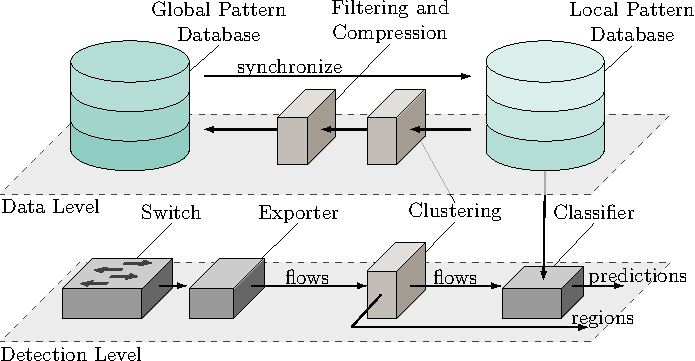
\includegraphics[width=0.8\linewidth]{tikz/high_level_architecture.pdf}
    \caption{Integration of the approach into a generic NIDS.}
    \label{fig:high_level_architecture}
\end{figure}



\subsection{Example Integration}\label{subsec:example_integration}
An exemplary integration of the CIDS into a generic NIDS is shown in Figure \ref{fig:high_level_architecture}. The shown NIDS consists of three components, which can be found on the detection layer. A flow exporter computes statistical flow features based on the network packets of a switch. A discriminative model serves as a classifier that operates on the specific feature set that the exporter extracts. After completing the training of a classifier instance on a given dataset, it is deployed within the detection pipeline. There, the classifier receives a stream of network flows and predicts them.

The CIDS mainly integrates at the data level, where the training data for the classifier is provided by the \textit{local pattern database}. At this point, the local pattern database only contains the \textit{local view} of the intrusion detection data from that particular member. In order to provide a global view for that member, a synchronization process between its local pattern database and the \textit{global pattern database} has to be initiated. Before the data is transferred to the global pattern database, is subject to a set of clustering, filtering and compression operations. This way, data privacy is maintained and the overhead is minimized by reducing the data volume. On the receiving side, the global pattern database combines data from all members to a global view.

Upon each update of the global pattern database, the new state of the global view is synchronized to each local pattern database and subsequently enhances the classifier on the detection level by extending the local intrusion detection dataset. Furthermore, an identical clustering operation as on the data level is applied on the detection level. Each incoming flow is assigned to a certain cluster, which is referred to as \textit{region}. While the predictions from the classifier are suitable for detecting attacks that are known to the CIDS, regions are leveraged for the detection of novel data patterns and similarity-based correlations that uncover stealthy attacks, which are executed on the resources of multiple CIDS members simultanously.

\subsection{Clustering}\label{subsec:clustering}

Since the results of the clustering operation should be consistent, while its execution is distributed among all members of the CIDS, an unsupervised algorithm with few parameters for initialization has to be selected. Additionally, the algorithm should be scalable, since it is to be applied on whole databases on the data level and on streams of live data on the detection level. Given these requirements, random projection is a good choice. 


By using random projection, real data points are clustered according to their angular distance. Furthermore, the projection result is a binary string, which can be used for storing similar data points into a common bucket of a hash table by using the binary string as an index. In the context of the generative pattern database, the combination of random projections and hash tables is exploited as the main controlling primitive for data persistence and retrieval. Instead of using randomly selected projection planes, a shared seed results in the application of a common projection function among all members of the collaboration. In other words, similar data points from different datasets are indexed to a common global bucket, i.e. region. Each region is subject to the transformations individually, which is utilized as a data parallelism mechanism. Thus, this approach is natively suited for cloud deployments where bursty workloads can be served effectively. Lastly, this mechanism enables a similarity-based correlation of distributed intrusion events. As incoming data is monitored on the detection level, the clustering is applied, which results in a pattern that can be used for novelty checks or global occurrences within the CIDS.

\subsection{Filtering and Compression}\label{subsec:filtering_and_compression}

Two types of data are extracted within individual regions. First, metadata of local datasets is collected by counting label occurrences, which serve as indicator for determining if the respective region needs to be subject to the second extraction type. Second, models that are trained with generative algorithms on local attack data are the exchange medium for disseminating information within the CIDS. This provides two main advantages. For one, no original data leaves a local network and therefore does not violate any privacy restrictions. For another, the data is compressed considerably by representing it in form of a generative model. 

\subsection{Global View}\label{subsec:global_view}

\begin{figure}[b!]
    \centering
    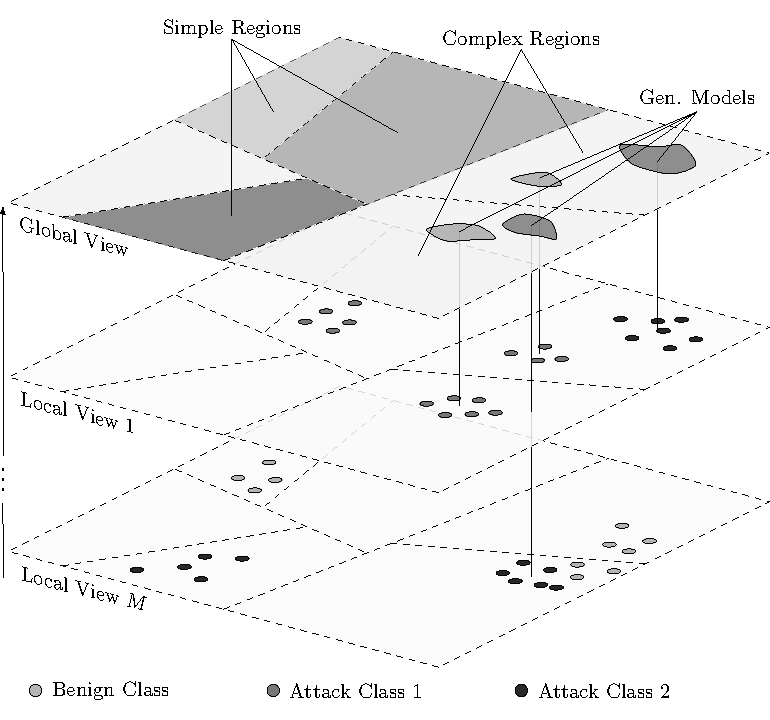
\includegraphics[width=0.8\linewidth]{tikz/global_view.pdf}
    \caption{Building the global view by combining $M$ local views.}
    \label{fig:global_view}
\end{figure}

\subsection{Creation}
As shown in Figure \ref{fig:global_view}, each view is partitioned by a common projection function into an identical set of regions. Each local view contains original datapoints from its respective dataset. In this example, there exist three different classes globally, which occur differently in each local dataset. Examining a specific region, the combination of unique classes within all local views determines its complexity on a global level. If a region contains more than one class, it potentially exhibits a non-linear decision boundary, hence it is called complex. Otherwise, a region is called simple. Attack data within a complex region, seperated by its label, is used as training data for a generative algorithm. Subsequently, the resulting model is transferred to the global view. 

\subsection{Usage}
A synchronization process disseminates the region complexity estimations and the generative models to all local views. By sampling data from multiple generative models, a synthetic dataset is assembled, which is blended into the respective local datasets for enhancing the subsequent training of a discriminative model.